% Chapter 4

\chapter{代码结果及实验验证}

我们分别采用手工构造和随机生成的数据对算法进行测试。

考虑到对凸多边形的三角划分有确定性的最优解,为了便于对比,我们的代码实现在所有子多边形均为凸多边形后即产生输出。

图\ref*{polygon}是手工构造的一组测试用例,具有大量互相嵌套,位置关系复杂的孔洞。我们将主要通过本组数据对算法进行测试。

\begin{figure}[htbp]
    \centering
    \begin{minipage}{0.4\textwidth}
        \centering
        
\includegraphics[width=0.95\textwidth]
        {figures/polygon.png}
        \caption{具有多个复杂孔洞的多边形}
        \label{polygon}
    \end{minipage}
    \begin{minipage}{0.4\textwidth}
        \centering
        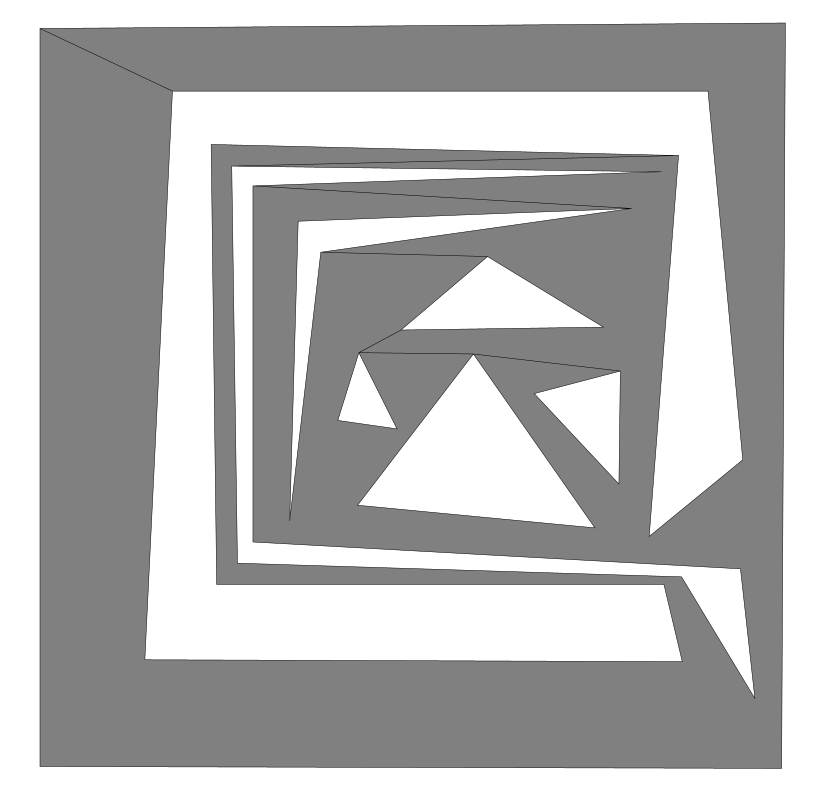
\includegraphics[width=0.95\textwidth]
        {figures/mergehole1.png}
        \caption{对多边形的孔洞进行消除}
        \label{mergehole}
    \end{minipage}
\end{figure}
首先,如图\ref*{mergehole},算法对多边形的所有孔洞进行合并。
通过数次切割,所有的内部孔洞通过一条宽度为0的桥与多边形外界相连,多边形的所有边界合并为一体,以便于接下来的处理操作。

在这一步,经测试发现,合并方式的不同对最终结果并没有非常大的影响。
究其原因是,略经优化后的朴素做法所选择的边并不会特别差;而少数相对较差的边即使在合并孔洞这一步未被选中,在接下来的初步分割或是最后的Delaunay三角网生成中仍然大概率作为一条切割边。而朴素算法相比于准确的计算出总长最短的切割边,可以较大程度的节省运算所耗时间。

在完成对多边形孔洞的合并之后,我们便可以开始对凹多边形进行分割了。在此步,我们的目标是将原有的凹多边形分割成相对数目较少的凸多边形,并通过控制~\ref*{sec:limit}中提到的修正值在效率和精准度之间做出平衡。

图\ref*{small},\ref*{large}是修正值分别取0.5和1时的分割结果。可以看到,修正值较小时,这一步的切分较为保守,可以保留下相对更规整的凸多边形,同时避免了一部分判断失误而产生的错误划分。算法在运行本测试用例时消耗时间仅需40毫秒,其中修正值取1时运行时间相比修正值取0.5时减少约3毫秒。

综合两图可以看到,经过这一步,多边形中的全部凹顶点均被分割为数个凸顶点,所有的多边形均被转化为凸多边形。接下来分别对每个位置调用Delaunay三角剖分算法即可得出最后对多边形三角化的结果。
\begin{figure}[htbp]
    \centering
    \begin{minipage}{0.4\textwidth}
        \centering
        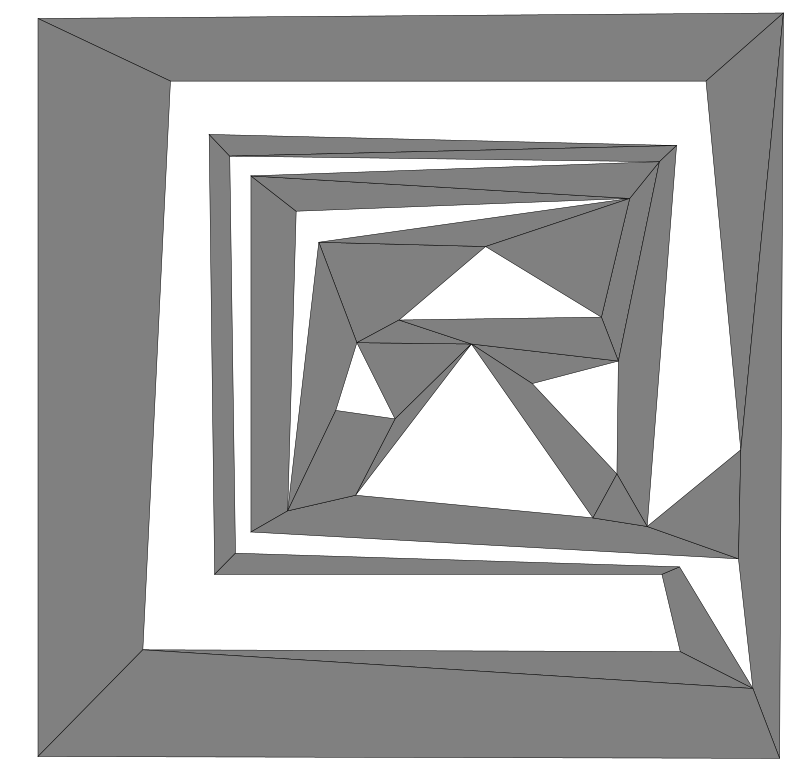
\includegraphics[width=0.95\textwidth]
        {figures/output2.png}
        \caption{取较小修正值的结果}
        \label{small}
    \end{minipage}
    \begin{minipage}{0.4\textwidth}
        \centering
        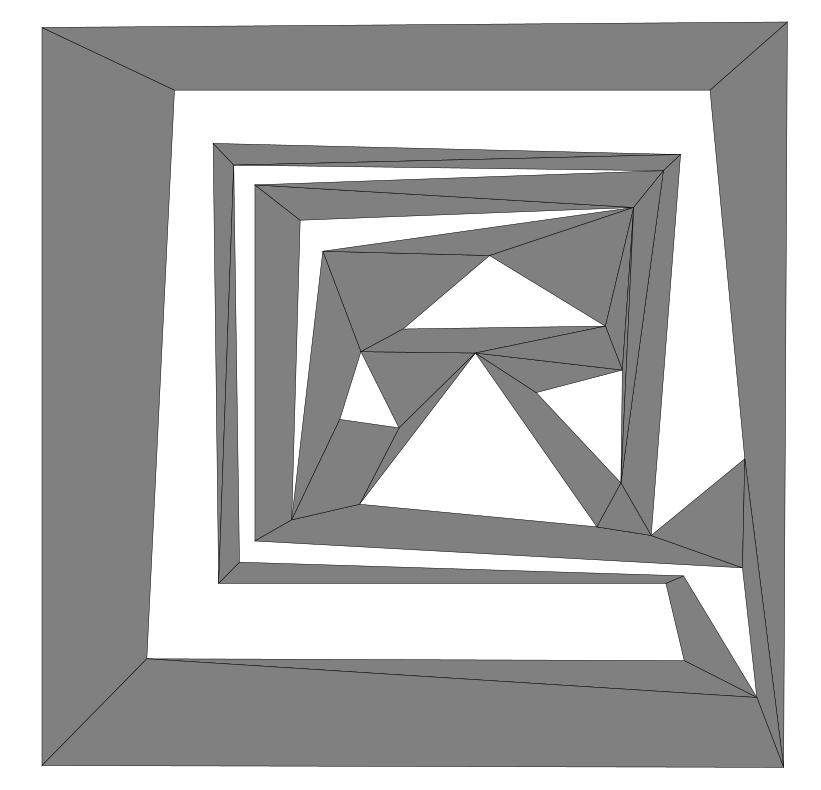
\includegraphics[width=0.95\textwidth]
        {figures/output1.png}
        \caption{取较大修正值的结果}
        \label{large}
    \end{minipage}
\end{figure}



与常用的耳切法等算法相比,本文的算法实现具有高效,准确,可自定义等多种优势,可以较好的解决多边形三角化的问题。



% 通过在顶点上添加桥边和辅助节点,我们可以通过一次切割联通两个多边形孔洞,或是将一个多边形孔洞与外界相连。如图~\ref*{merge}所示,在添加额外的两个顶点和两条边后,两个多边形孔洞的边界将会合并为一个连续的环,而其代表的多边形区域不发生改变。由此,通过数次合并后,原有的带孔多边形将变为不含孔洞的凹多边形。
% \section{预处理}
% 为确保多边形孔洞合并后点的顺序正确,边界不产生交叉,需要提前对多边形孔洞的顶点方向进行预处理。

% 我们令多边形外圈的点以逆时针顺序排列,内圈孔洞则以顺时针顺序排列。如此处理之后,两个多边形孔洞在合并时将保持正确的旋转方向,避免边界出现交叉。

% \begin{figure}[htp]
%     \centering
%     \includegraphics[width=0.5\textwidth]
%     {figures/mergehole.png}
%     \caption{正确处理多边形旋转顺序后的合并}
%     \label{merge}
%   \end{figure}

% \section{朴素的合并方式}
% 将多边形上的所有点按照x坐标从小到大为第一关键字,y坐标从大到小为第二关键字排序。
% 按顺序遍历所有顶点,并记录当前已经遍历的所有节点所属的边界。
% 当新遍历到的顶点所属的边界与之前的边界未进行过合并时,选择之前遍历过的顶点之中与当前点距离最近的顶点,向其延伸一条射线,并于第一段相连的多边形边界处相连。以此线段作为切割线,合并相关联的两个边界。

% 遍历多边形上的所有节点后,多边形的每个孔洞都直接或间接的与多边形外边界相连,因此我们便可以消除多边形内部的孔洞。
% \section{对上述算法的改良}
% 借助最小生成树的思路,我们可以最小化切割边的总长度。

% 枚举多边形中的每对分属两个不同多边形孔洞的点对,并判断其连线是否与其他边冲突,记录所有合法的切割边。

% 将切割边按长度从小到大排序,按顺序处理边。对于每条切割边,若切割边所连接的两部分多边形未被合并,且该边与已有的切割边之间不产生冲突,则沿此切割边将两侧的多边形边界合并为一体。当选择的切割边数目恰好与多边形孔洞数目相等时,所有的多边形边界均合并完成,原多边形的孔洞消除完成。

% \section{采用分治法合并孔洞}
% 我们可以采用分治计算Delaunay triangulation算法中的思想,使用相似的方法完成对孔洞的合并。

% 首先将多边形孔洞的所有点按照x坐标从小到大为第一关键字,y坐标从大到小为第二关键字排序。接下来每次将待处理的点集分为左右两半,递归合并点集中的不同多边形片段。

% 当点集中的点不多于两个时,递归终止。若点集中的点分属不同多边形,则添加一条新的切割边连接两个顶点,将其加入候选集合。

% 接下来我们处理两个点集答案的合并。

% 从原多边形孔洞的边集中搜索,判断是否存在原有的连接两半点集的边。

% 若不存在这样的边,则使用分治计算Delaunay triangulation算法中的计算方式,找出所有合法的LR-edge,在候选集合中修正与之冲突的切割边,并额外添加一条最短的LR-edge至集合中。此处的合法LR-edge计算方式与分治计算Delaunay triangulation算法中的相似,但是寻找可行端点时需要排除连边时会与原多边形中已有的边产生冲突的顶点。

% 若存在连接两半点集的边,则将其直接加入集合,在候选集合中删除与之冲突的切割边,并寻找一条额外的切割边,连接原切割边所连接的集合。

% 由此思路,即可完成对所有孔洞的合并。接下来取孔洞中与边界距离最短的点对相连即可将多边形的孔洞消除。
% \section{代码}
% \subsection{原始代码}
% 朴实的代码块:

% 使用verbatim可以得到原样的输出,如下:

% \begin{verbatim}
%     print("Hello world!")
% \end{verbatim}

% 使用\href{https://en.wikibooks.org/wiki/LaTeX/Source_Code_Listings}{listings}环境可以对代码进行进一步的格式化,如下:

% \lstset{basicstyle=\ttfamily,breaklines=true}
% \begin{lstlisting}[language=Python,frame=single]
% import numpy as np

% a = np.zeros((2,2))
% print(a)
% \end{lstlisting}

% \subsection{代码高亮}
% 还可以对代码进行高亮,请参考 \href{https://www.overleaf.com/learn/latex/Code_Highlighting_with_minted}{Code Highlighting with minted}。
% 请先到cls文件中启用minted库。
% 注意使用Minted库时,需要系统默认Python有Pygments库,可以通过\verb|$ pip install Pygments| 来进行安装。且需要在编译时加上\verb|--shell-escape|参数,否则会报错。

% \usemintedstyle{vs}
% \begin{minted}[linenos,baselinestretch=1.0,frame=lines]{cpp}
% #include <iostream>
% using namespace std;

% int main() 
% {
%     cout << "Hello, World!";
%     return 0;
% }
% \end{minted}

% \subsection{算法描述/伪代码}
% 参考 \href{https://en.wikibooks.org/wiki/LaTeX/Algorithms}{Algorithms},下面是一个简单的示例:

% \begin{algorithm}[H]
%   \setstretch{1.5} % 代码间行距设定
%   \SetAlgoLined
%   \KwResult{Write here the result }
%    initialization\;
%    \While{While condition}{
%     instructions\;
%     \eIf{condition}{
%      instructions1\;
%      }{
%      instructions3\;
%     }
%    }
%   \caption{How to write algorithms}
% \end{algorithm}

% \begin{algorithm}[]
%   \SetKwInOut{Input}{输入}
%   \SetKwInOut{Output}{输出}
%   \caption{\sc DeepWalk\((G, w, d, \gamma, t)\)}\label{DeepWalk}
%   \Input{图\(G(V,E)\) \\
%     窗大小\(w\) \\
%     嵌入维度\(d\) \\
%     每个节点游走数\(\gamma\) \\
%     游走距离\(t\)
%   }
%   \Output{节点表征矩阵\(\Phi\in\mathbb{R}^{|V|\times d}\)
%   }
%   初始化:从\(\mathcal{U}^{|V|\times d}\)采样\(\Phi\) \\
%   从\(V\)建立二叉树\(T\) \\
%   \For{\(i=0\) to \(\gamma\)}{
%     \(\mathcal{O}\) = Shuffle(\(V\)) \\
%     \ForEach{\(v_i\in\mathcal{O}\)}{
%       \(\mathcal{W}_{v_i}=RandomWalk(G, v_i, t)\) \\
%       \(\textsc{SkipGram}(\Phi, \mathcal{W}_{v_i}, w)\)
%     }
%   }
% \end{algorithm}

% \section{绘图}

% 关于使用 \LaTeX{} 绘图的更多例子,请参考 \href{https://www.overleaf.com/learn/latex/Pgfplots_package}{Pgfplots package} 中的例子。
% 一般建议使用如Photoshop、PowerPoint等制图,再转换成PDF等格式插入。

% \section{写在最后}
% 工具不重要,对工具的合理运用才重要。希望本模板对大家的论文写作有所帮助。
